%!TEX encoding = UTF-8 Unicode  
\documentclass{article}  
\usepackage{xeCJK}
\setCJKmainfont[BoldFont=STZhongsong, ItalicFont=STKaiti]{STSong}
\setCJKsansfont[BoldFont=STHeiti]{STXihei}
\setCJKmonofont{STFangsong}
\usepackage{graphicx}
\usepackage{amsmath}
 \usepackage{clrscode}
\usepackage{listings}

\lstset{language=C++}%这条命令可以让LaTeX排版时将C++键字突出显示

\lstset{breaklines}%这条命令可以让LaTeX自动将长的代码行换行排版

\lstset{extendedchars=false}%这一条命令可以解决代码跨页时,章节标题,页眉等汉字不显示的问题




\begin{document}  

\title{文献综述}
\date{}

\maketitle


\textbf{一、背景介绍}
      \qquad
\newline
      \qquad
      近年来,在工程应用中,求解高阶矩阵的需求日益增长,全矩阵运算脱离了实际的硬件限制,为了满足这一日益增长的需求,同时这些矩阵通常都有着一个特征——非零元远少于零元,稀疏矩阵这门学科便应运而生。
在 20 世纪 60 年代研发电子网络的电子工程师们是最早的去利用稀疏性来应用稀疏矩阵进行工程上的计算的。[1]
而在微分方程数值解、线性规划等的有限元分析中,经常出现求解高阶稀疏线性方程组,如利用全矩阵进行存储,则需要$n^2$的空间复杂度和$n^3$的乘法运算时间复杂度,显然,这种程度的运算量是无法被微型计算机,甚至是工作站所接受的。
而利用矩阵的稀疏性,可以有效地减小消耗很多无谓的存储空间以及无谓的计算,在很大的程度上降低了时间和空间复杂度,降低了计算对硬件的需求,使计算成为可能。
\newline
二、国内外研究现状\newline
1、研究方向及进展\newline

在这些年的发展中,出现了很多的存储方法,比如:对角线存贮法、对称矩阵的变带宽存贮法、坐标存贮法、Elipack-Itpack存贮法、CSR存贮法、Shermans存贮法、超矩阵存贮法、动态存贮方案等[2]。
\newline
如行压缩存储方式(Compressed Row Storage):
CRS存储可以高效地存取任意一行非零元素,但存取任意一列非零元则需要遍历整个CRS存储结构。相应地,与CRS存储的稀疏矩阵相关的算法要高效的编程实现,算法的计算顺序必须按行来进行。[e]
下面对应于CRS存储:
\newline\newline\newline\newline\newline\newline\newline

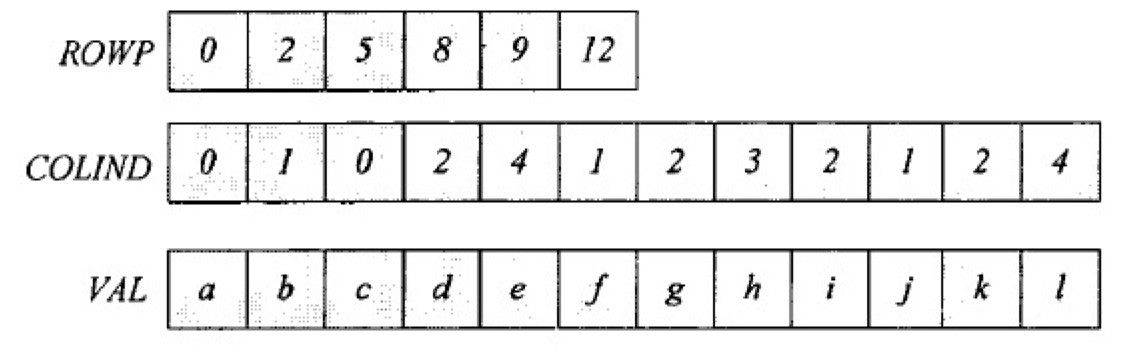
\includegraphics[scale=0.25]{crs.png}
我们可以发现,ROWP数组存储的时行非零元的增长量。COLIND则存储的是列索引值,典型的C语言结构实现为\newline

\begin{lstlisting}

struct cr_matrix{ 
	int *Ri;/*col index*/ 
	int *Rp;/*length nrow+1*/ 
	double *Rx; 
	int Rncol;
	int Rnrow;
};

\end{lstlisting}


在早期计算机时,串行的算法占到主流,自然,稀疏矩阵的存储方式以及稀疏矩阵的计算都是为了串行算法服务的。但是随着计算机的发展,计算机集群、多核CPU、GPU并行等的出现,让并行算法在计算时间上远远地超越了串行算法,为了更好的适应并行计算中的稀疏矩阵计算,出现了许多新的算法以及存储方式。例如对于非结构化的矩阵,基于CUDA框架下的SCOO形式的SpMV算法比利用基于Cusp库的SCOO具有更高的效率。[y]
\newline
而在做稀疏矩阵的计算时,通常都是做一系列的基本运算,如:矩阵转置、矩阵向量乘法、矩阵矩阵乘法、数乘等。为了能得到更好的效率,许多研究者致力于寻找对于这些计算最优的存储结构及计算算法,同时提供了许多类库供科学计算使用,如:Portable, ExtensibleToolkit for Scientific Computation(PETSc)、Boost、GNU Scientific Library (GSL)等。\newline
例如,在Boost-uBLAS中有着稀疏矩阵的模板mapped\_matrix<T, F, A>(元素映射矩阵存储形式)、compressed\_matrix<T, F, IB, IA, TA>(压缩存储格式)、coordinat\_matrix<T, F, IB, IA, TA>(坐标存储格式)。
分别有着如下示例:[h]\newline
\textbf{mapped\_matrix:}
\begin{lstlisting}

#include <boost/numeric/ublas/matrix_sparse.hpp>
#include <boost/numeric/ublas/io.hpp>

int main () {
    using namespace boost::numeric::ublas;
    mapped_matrix<double> m (3, 3, 3 * 3);
    for (unsigned i = 0; i < m.size1 (); ++ i)
        for (unsigned j = 0; j < m.size2 (); ++ j)
            m (i, j) = 3 * i + j;
    std::cout << m << std::endl;
}

\end{lstlisting}

\textbf{compressed\_matrix:}
\begin{lstlisting}

#include <boost/numeric/ublas/matrix_sparse.hpp>
#include <boost/numeric/ublas/io.hpp>

int main () {
    using namespace boost::numeric::ublas;
    compressed_matrix<double> m (3, 3, 3 * 3);
    for (unsigned i = 0; i < m.size1 (); ++ i)
        for (unsigned j = 0; j < m.size2 (); ++ j)
            m (i, j) = 3 * i + j;
    std::cout << m << std::endl;
}

\end{lstlisting}

\textbf{coordinate\_matrix:}
\begin{lstlisting}

#include <boost/numeric/ublas/matrix_sparse.hpp>
#include <boost/numeric/ublas/io.hpp>

int main () {
    using namespace boost::numeric::ublas;
    coordinate_matrix<double> m (3, 3, 3 * 3);
    for (unsigned i = 0; i < m.size1 (); ++ i)
        for (unsigned j = 0; j < m.size2 (); ++ j)
            m (i, j) = 3 * i + j;
    std::cout << m << std::endl;
}
\end{lstlisting}

在多年的研究中,各种相关的研究成果页层出不穷,例如,
根据Michele Martone的研究成果,在对称矩阵乘法,或者转置的矩阵向量乘法中,RSB格式的迭代算法效率是比较高的[x]。
而在李佳佳,张秀霞,谭光明,陈明宇的研究中,得到了影响矩阵性能的参数集,可以利用该参数集提取矩阵特征,并输出最优存储格式,供数值解法器和上层应用调用。[a]
为了适用于大数据集计算以及克服现有稀疏矩阵乘法算法低效的问题,郑建华,朱 蓉,沈玉利提出了一种基于向量线性组合(VLC)的矩阵乘法处理模式,同时采用MapReduce计算模型实现了基于VLC模式的并行矩阵乘法算法。[d]
而在集群计算方面,负载平衡是不能不提到的,为了更好地发挥集群计算的计算能力,付朝江博士给出了基于贪婪分配的稀疏矩阵与向量乘的负载平衡的解决方案。[b]
\newline

2、存在问题\newline

稀疏矩阵的存储没有一种通用的形式,各种形式都各有利弊[f],这也就需要我们对于不同的情况去寻找最合适的存储形式来计算,虽然李佳佳,张秀霞,谭光明,陈明宇[a]的研究得到了一个参数集用以寻找最优存储形式,但是比较的存储形式比较少,还有多种形式没有计入考量范围。
\newline
而在超大规模的稀疏矩阵计算时,计算机的内存可能不能完全存储这些数据,部分数据将会存储在硬盘中,而硬盘的读取效率远低于内存,如何更好地将硬盘中的数据读取到内存中,减少内存与硬盘交互的时间,同时,如何降低内存与缓存间的交互时间也是一个问题。
\newline
而随着计算机的普及,计算机进入了家家户户,分布式计算逐渐成为可能,让普通的计算机使用者参与到科学计算中,贡献GPU资源来帮助研究人员更快地完成计算,但是这尚未得到普及,同时,中国尚未形成一个成熟的分布式计算平台,也没有培养出普通用户参与到分布式计算项目的习惯。\newline



3、研究展望\newline
为了更好的适应现代的工程计算需求,计算更大规模的稀疏矩阵,以及适应新的CPU指令集和GPU计算框架,稀疏矩阵的存储形式值得进一步的研究。同时,伴随着分布式计算的发展,更为高效的冗余计算机制和任务分配机制也将会带给稀疏矩阵计算新的研究方向。
按照摩尔定律,计算机的计算能力将毎隔18-24个月翻一番,那么计算稀疏矩阵的能力也将相应提高。同时随着量子计算机、光计算机等的出现,更高德计算能力也将随之到来。而为了更好地发挥这些硬件的能力,以往的算法可能并不再适合了,需要开发新的算法以适应新的硬件。而对于硬件商而言,如Intel、AMD等CPU厂商而言,封装更多的CPU指令,让用户可以直接调用CPU指令来进行科学计算,更好地发挥硬件的性能。对于普通计算机用户,培养参与到分布式计算的习惯,通过建立一个国家级的分布式计算中心,建立奖励机制,鼓励普通计算机用户参与到分布式计算中,为研究计划中的稀疏矩阵计算贡献自己的计算资源。\newline

\textbf{三、参考文献}
      \qquad
\newline
 [1]Yousef Saad.Iterative Methods for Sparse Linear Systems[M].SECOND EDITION.USA:Society for Industrial and Applied Mathematics,2003年.68.\newline
 [2]张永杰、孙秦.稀疏矩阵存储技术[J].长春理工大学学报,2006年,03期:38-41.\newline
  [x]Michele Martone.Efficient multithreaded untransposed, transposed or symmetric sparse matrix–vector multiplication with the Recursive Sparse Blocks format[J].Parallel Computing, 2014,40:47-58.\newline
   [y]Hoang-Vu Dang,  Bertil Schmidt.CUDA-enabled Sparse Matrix–Vector Multiplication on GPUs
using atomic operations[J].Parallel Computing, 2013,Vol.39 (11):737-750.\newline
  [a]李佳佳,张秀霞,谭光明,陈明宇.选择稀疏矩阵乘法最优存储格式的研究[J].计算机研究与发展 , Journal of Computer Research and Developmen,2014年,04期:882-894.\newline
[b]付朝江.基于贪婪分配的稀疏矩阵与向量乘的负载平衡[J].福建工程学院学报 ,2010年,01期:79-82.\newline
[d]郑建华,朱 蓉,沈玉利.Sparse matrix multiplication algorithm based on MapReduce[J].仲恺农业工程学院学报,2013年,03期:45-50.\newline
[f]张永杰,孙秦.稀疏矩阵存储技术[J].长春理工大学学报,2006年,03期:38-41.\newline
 [e]冯广祥. 大型稀疏矩阵直接求解算法的研究及实现[D].  东北大学:系统工程,2010.\newline
 [h]Joerg Walter and Mathias Koch.Boost 1.57.0 Library Documentation-uBLAS. http://www.boost.org/doc/libs/1\_57\_0/libs/numeric/ublas/doc/index.html, 2011\newline
\end{document}  
